\chapter{Eulerian Graphs}

\section{Relevant Definitions}

\begin{definition}[Walk]
  A \textit{walk} in a graph is a sequence of the form \(v_1, e_1, v_2, e_2,
  ..., v_r\) for some \(r > 1\) where the \(v_i\)'s are vertices and the
  \(e_i\)'s are edges from \(v_i \to v_{i+1}\) for each \(1 \leq i < r\).
\end{definition}

\begin{remark}
  If \(r = 1\), then the walk consists of a single vertex and no edge. This is
  still valid.
\end{remark}

\begin{definition}[Trail]
  A \textit{trail} is a walk in which no edge appears more than once.
\end{definition}

\begin{definition}[Path (Alt.)]
  A \textit{path} is a walk in which no vertex appears more than once
\end{definition}

\section{Eulerian Graphs}

\begin{definition}[Eulerian Graphs]
  A connected graph \(G\) is \textit{Eulerian} if there exists a closed trail
  containing every edge of \(G\). This is also known as an \textit{Eulerian
  Circuit}. Note that this requires each edge to be traversed only once.
\end{definition}

\begin{definition}[Semi-Eulerian Graphs]
  A non-Eulerian graph \(G\) is \textit{semi-Eulerian} if there exists a trail
  containing every edge of \(G\). This is also known as an \textit{Euler Trail}.
\end{definition}

\begin{figure}[ht]
  \begin{center}
    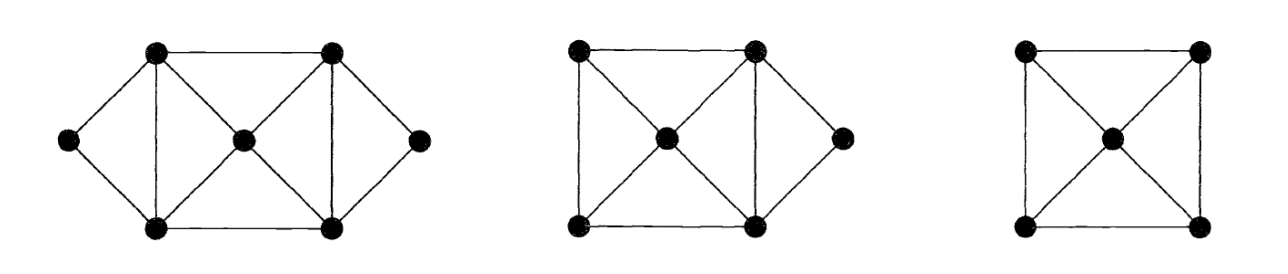
\includegraphics[width=0.69\textwidth]{figures/l02/eulerian-graphs}
  \end{center}
  \caption{(Left to right, respectively) Eulerian, semi-Eulerian, and non-Eulerian graphs}\label{fig:eulerian-graphs}
\end{figure}

\begin{theorem}[Euler, 1736]
  A connected graph \(G\) is Eulerian if and only if the
degree of each vertex of \(G\) is even.
\end{theorem}

\begin{proof}
  First, we will show the forward case: If a connected graph \(G\) is
  Eulerian---that is, it has an Euler circuit, then the degree of each vertex is
  even. Suppose that \(P\) is an Euler circuit. Whenever \(P\) passes through a
  vertex (except for the start and end vertices), it contributes 2 edges to said
  verted. Since each edge occurs exactly once, each vertex must have an even
  degree.

  Now, we will show the converse case: If each vertex in connected graph \(G\) has an even degree, then \(G\) has an Eulerian circuit. We will show this by induction on the number of edges of \(G\). First, claim that \(G\) has a cycle \(C\). We know this to be true since \(G\) is connected and each vertex has degree at least 2. Then, we remove edges of \(C\) from \(G\). We call this new graph \(H\). Note that \(H\) is possibly disconnected. Then, claim that each component of \(H\) has an Euler circuit. By applying induction on the number of edges, we still have that each vertex still has even degree. Next, create an Euler circuit of \(G\) by :
  \begin{itemize}
    \item Following the edges of \(C\)
    \item If we reach \(H\), then trace the circuit of that component of \(H\) and finish where you started
    \item We continue until we reach the initial vertex of \(C\)
  \end{itemize}
\end{proof}

\section{Fleury's Algorithm}


